%!TEX TS-program = xelatex
\documentclass[]{friggeri-cv}
\usepackage{afterpage}
\usepackage{hyperref}
\usepackage{color}
\usepackage{xcolor}
\hypersetup{
    pdftitle={},
    pdfauthor={},
    pdfsubject={},
    pdfkeywords={},
    colorlinks=false,       % no lik border color
   allbordercolors=white    % white border color for all
}
\addbibresource{bibliography.bib}
\RequirePackage{xcolor}
\definecolor{pblue}{HTML}{0395DE}

\begin{document}
\header{Josué }{Gutiérrez}
      {Computer Engineer}
      
% Fake text to add separator      
\fcolorbox{white}{gray}{\parbox{\dimexpr\textwidth-2\fboxsep-2\fboxrule}{%
.....
}}

% In the aside, each new line forces a line break
\begin{aside}
    ~
    ~
    ~
    ~
    ~
  \section{Phone}
    +34 664 84 31 37
    ~
  \section{e-Mail}
    \href{mailto:contacto@josuegutierrez.es}{contacto@\\josuegutierrez.es}
    ~
  \section{Web \& Git}
    \href{http://www.josuegutierrez.es}{josuegutierrez.es}
    \href{https://github.com/JoxuMac}{github.com/joxumac}
    ~
  \section{Programming}
    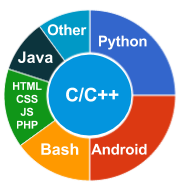
\includegraphics[scale=0.62]{img/programming.png}
    ~
  \section{S.O.}
    \textbf{MacOS}
\includegraphics[scale=0.40]{img/5stars.png}
    \textbf{Windows}
\includegraphics[scale=0.40]{img/4stars.png}
    \textbf{GNU/Linux}
\includegraphics[scale=0.40]{img/3stars.png}
    ~
  \section{Skills}
    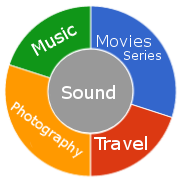
\includegraphics[scale=0.62]{img/personal.png}
    ~
    \section{Languages}
    \textbf{Spanish}
\includegraphics[scale=0.40]{img/5stars.png}
    \textbf{English}
\includegraphics[scale=0.40]{img/3stars.png}
    ~
\end{aside}

\section{Experience}
\begin{entrylist}
  \entry
    {09/17 - Now}
    {Talentum Scholarship 2017}
    {Furious Koalas Interactive \& Telefonica}
    {Beneficiary of the Telefónica Talentum Grant with the company Furious Koalas. Design team in the ARMov project of Augmented Reality.\\}
  \entry
    {11/17}
    {Volunteer 1st Week Computer Vision}
    {UCLM, ESI \& VISILAB}
    {Volunteer in the 1st Week of the Vision by Computer, Project ref. FCT-1611257, with the collaboration of the Spanish Foundation for Science and Technology Ministry of Economy, Industry and Competitiveness, UCLM, School of Informatics and VISILAB.\\}
    \entry
    {05/17}
    {1 Award – CTF Hackbits}
    {UCLM, ESI, Hackbits \& Cirebits}
    {Winner of the First Place in the CTF (Capture of Flag) of cybersecurity organized by HackBits.\\}
\end{entrylist}

\section{Education}
\begin{entrylist}
  \entry
    {2014 - Now}
    {Informatics Engineering}
    {Castilla-La Mancha University}
    {The School of Computer Science of CR seeks the training of professionals capable of designing, managing and maintaining systems, applications or products that allow the generation, support, storage, transmission or organization of information, with full knowledge of the methods and techniques involved.}\\
\end{entrylist}

\section{Certifications}
\begin{entrylist}
  \entry
    {07/2015}
    {CCNA Exploration: Network Fundamentals}
    {Cisco Networking Academy}
    {\emph{\\}}
    \entry
    {04/2015}
    {TOEIC Listening \& Reading}
    {Capman ETS Toeic}
    {\emph{590 Points TOEIC.\\}}
    \entry
    {04/2015}
    {Smact Avanttic Workshop}
    {\begin{flushright}Castilla-La Mancha University \& \\Avanttic Technological Consulting S.L.\end{flushright}}
    {\emph{First edition of avanttic \_day, as a continuation of the Big Data conference held by the Higher School of Information Technology.}}
\end{entrylist}
\end{document}
